%%%%%%%%%%%%%%%%%%%%%%%%%%%%%%%%%%%%%%%%%%%%%%%%%%%%%%%%%%%%%%%%%%%%%%%%%%
%
%   UNIVERSITY OF YORK LAB REPORT TEMPLATE
%
%   Requirements: 
%     To compile, you must also have a copy of the style file 
%		YorkLabReport.sty 
%     
%   Author: Chris Harte
%   
%   Version 1.0
%
%   Date: December 2014
%
%   Notes:
%     This is intended as a template for a short lab report, not a final
%     project report/thesis. 
%
%%%%%%%%%%%%%%%%%%%%%%%%%%%%%%%%%%%%%%%%%%%%%%%%%%%%%%%%%%%%%%%%%%%%%%%%%%

%%%%%%%%%%%%%%%%%%%%%%%%%%%%%%%%%%%%%%%%%%%%%%%%%%%%%%%%%%%%%%%%%%%%%%%%%%
% DOCUMENT CLASS DECLARATION:
% Set the document class to two-sided A4 paper using the style "report"
\documentclass[a4paper,twoside, 10pt]{report}
%%%%%%%%%%%%%%%%%%%%%%%%%%%%%%%%%%%%%%%%%%%%%%%%%%%%%%%%%%%%%%%%%%%%%%%%%%

%%%%%%%%%%%%%%%%%%%%%%%%%%%%%%%%%%%%%%%%%%%%%%%%%%%%%%%%%%%%%%%%%%%%%%%%%%
% INCLUDED PACKAGES:
% List any required packages below.  In the case of this template we only
% require the accompanying YorkLabReport.sty style file because it contains
% a list of required packages and thus keeps this file tidy.
\usepackage{YorkLabReport}
%%%%%%%%%%%%%%%%%%%%%%%%%%%%%%%%%%%%%%%%%%%%%%%%%%%%%%%%%%%%%%%%%%%%%%%%%%

%%%%%%%%%%%%%%%%%%%%%%%%%%%%%%%%%%%%%%%%%%%%%%%%%%%%%%%%%%%%%%%%%%%%%%%%%%
% COMMANDS AND DEFINITIONS:
%
% This defines a new command called \code{} that takes one argument. The 
% command sets the font of its argument text to be \texttt{}.  This gives 
% "teletype" style text i.e. a monospaced serif font like courier
\newcommand{\code}[1]{\texttt{#1}}
%
% This line stops the section numbers from including a redundant chapter number: 
\renewcommand*\thesection{\arabic{section}}
%%%%%%%%%%%%%%%%%%%%%%%%%%%%%%%%%%%%%%%%%%%%%%%%%%%%%%%%%%%%%%%%%%%%%%%%%%

%%%%%%%%%%%%%%%%%%%%%%%%%%%%%%%%%%%%%%%%%%%%%%%%%%%%%%%%%%%%%%%%%%%%%%%%%%
% 
% BEGIN THE BODY OF THE DOCUMENT
%
%%%%%%%%%%%%%%%%%%%%%%%%%%%%%%%%%%%%%%%%%%%%%%%%%%%%%%%%%%%%%%%%%%%%%%%%%%
\begin{document}

    % YOUR REPORT TITLE:
    \title{Flocking Behaviour Simulation}

    % YOUR SUBTITLE 
    \subtitle{Java Programming Assessment 2014/15 -- ELE0005C}
    
    %YOUR NAME OR CANDIDATE NUMBER 
    % (depending on whether the report is being enonymously marked) 
    \author{Y3508038}
    
    % THE DATE OF THE REPORT
    \date{\today}

% \maketitle takes all the fields we just filled in and builds a title 
% page with them.
\maketitle

% table of contents page with a quote and abstract
\tableofcontents 
\vfill

\begin{quotation}
\textit{``No product of human intellect comes out right the first time. We rewrite sentences, rip out knitting stitches, replant gardens, remodel houses, and repair bridges. Why should software be any different?''}~--~Ruth Wiener~\cite{Wiener93quote}
\end{quotation}

\vfill
\section*{Abstract}
This report will cover the planning, development and implementation of flocking behaviour in \textsc{Java}, and assumes the reader to have basic-to-intermediate knowledge in the \textsc{Java} programming language. The result is a fully functioning flocking simulator which fits the specifications but is open for improvement.

\vfill
\newpage

%contents page ended





%----------------------
\section{Introduction}
\label{sec:intro}

The human race has always been fascinated by nature, and by studies we have learned a great deal about nature and its processes. Technology is advancing steadily, and implementations of nature phenomena in research and science has been of great help for researchers and developers. One of these scientists, Craig W. Reynolds, published an article in 87~\cite{reynolds87behavioral} on the phenomena of flocking organisms. He wrote about the phenomenon and its \textit{then} non-existent implementation in code, as well as his suggestion to how it could be done. This report will cover the proceedings of my own implementation of a flocking simulation written in \textsc{Java}. 

\section{Specifications}
\label{sec:specification}

The assignment set some specifications for the application. The application must:
\begin{itemize}
	\item be written in \textsc{Java}
    \item use modular and object-oriented coding and handle errors in a robust fashion
    \item simulate a number of flocking 'robots' that exist in a 2-dimensional world displayed graphically on the computer screen
    \item allow for the number of robots and their initial positions to be set by the user~(by GUI elements or by file input/output or both)
\end{itemize}

Additional features could be: 
\begin{itemize}
	\item adding other objects into the world(such as predators, obstacles etc)
\end{itemize}




%----------------------
\section{Analysis}
\label{sec:analysis}
Flocking birds, as stated by C. W. Reynolds~\cite{reynolds87behavioral} and several other sources~\cite{Hemelrikj11CausesOfFlocks, Wiki15Flocking}, are not made up by anything else than $n$ individuals taking their own individual decisions based on their surroundings. The flocks fluidity and apparent singularity is therefore just an illusion. Flocking birds use three simple ``rules'' to decide on their next step, and sum of the rules can be thought of as the birds acceleration. The rules can be written as follows~\cite{reynolds87behavioral}:

\begin{enumerate}
  \item Collision Avoidance~(\textit{Separation}): attempt to avoid collisions with nearby birds~(close range)
  \item Match velocity~(\textit{Alignment}): attempt to match the velocity of nearby birds
  \item Flock Centering~(\textit{Cohesion}): attempt to fly towards the average position of nearby birds
\end{enumerate}

\begin{figure}[H]
  \centering{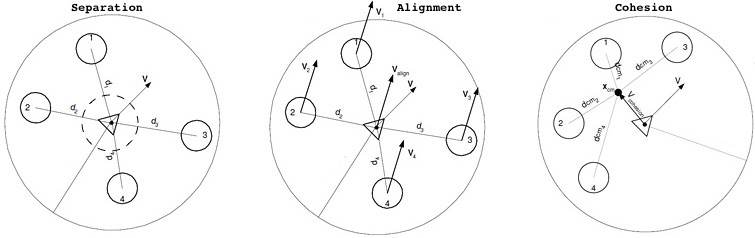
\includegraphics[width = \textwidth]{images/flocking_rules.jpg}}
  \abovecaptionskip
  \belowcaptionskip
  \caption{Graphical Explanation of the Flocking Rules~\cite{reynolds87behavioral, unknown15flockingrules}}
  \label{fig:rules}
\end{figure}

\subsection{Simulation
\label{subsec:simulation}}

\begin{description}
	\item \textit{\textbf{Simulation} is the imitation of the operation of a real-world process or system over time~\cite{wiki15simulation}}
    \item \textit{\textbf{Boid} -- short for Bird-oid -- bird-like object~\cite{wiki15Boids})}
\end{description}

The behaviour will be simulated by having a world where one frame is equal to one update and a pause in the world. The next frame comes when the world is updated and paused another time, and so on. Preferably, a frame rate of 60$/s$ or more would make a smooth simulation, whereas frame rates below 30$/s$ is not wanted at all as the simulation would seem ragged and spastic. Instead of birds I will be simulating \textit{boids}, and a simulation capable of having around a hundred boids at once without major performance issues is what is aimed for.




%%----------------------
\section{Design}
\label{sec:design}
The application will consist of several levels of abstraction, and it might split into four parts. Mainly it will consist of the graphical user interface(GUI) where the user can watch and interact with the simulation. ``Behind'' the GUI there will be a ``world'' where the actual simulation will run, thus the GUI can be considered merely a graphical representation of the simulation. The boids will ``live'' in the world and interfere with each other solely affected by the rules of flocking mentioned earlier~(\ref{fig:rules}). Since it is desirable to add more than just the basic flocking, ``extra'' features can be added, see Table~\ref{tab:features}. Depending on what is implemented, the application will use only a small amount of inputs, and will most likely be limited to mouse events and possible file handling. 

\begin{table}[h]
\centering
  \begin{tabular}{l|c|l}
    Function 		& Specified & Task	\\\hline
    Play/Pause 		& JButton & Play and pause the Simulation	\\
    Reset 			& JButton & Reset the game to start-up conditions		\\
    Add (+) boids 	& JButton & Randomly place n boids in the simulation	\\
    Sub (-) boids 	& JButton & Remove the n last boids from the simulation 	\\
    Load 			& JButton & Save the current session to a .txt file		\\
    Save 			& JButton & Load a saved session						\\
    Watch over nBoids & JLabel & Monitors the total number of boids			\\
    Influence slider(s)	 & 3*JSlider & Setting the boids influence of each rule	\\
    FPS slider 		& JSlider 		& Set the Frame Rate per Second			\\
    Mouse click implementation  	& MouseListener & Add  one boid each mouse click	\\
    Monitor size-change & ComponentListener & Monitors the size of the world to	\\
  \end{tabular}
  \caption{Possible Features to be Added}
  \label{tab:features}
\end{table}

\begin{minipage}[T]{0.3\textwidth}
  \subsection{The GUI}
  \label{subsec:GUI}
  The GUI itself will consist of a JFrame with two JPanels placed onto it. The application will need to be ran or be started from a static context, which will be done from the \code{main} located in \code{MainFrame}. One of the JPanels will as said display the boids, and the second will act as an options panel for interaction with the world. The simulation is located in a separate simulation manager, done to be coherent with object-oriented programming. It is in the simulation the boids will actually live and interact, see figure~\ref{fig:idea}.
\end{minipage}
%
\begin{minipage}[C]{0.70\textwidth}
  \captionsetup{type=figure}
  \begin{figure}[H]
    \hfill
    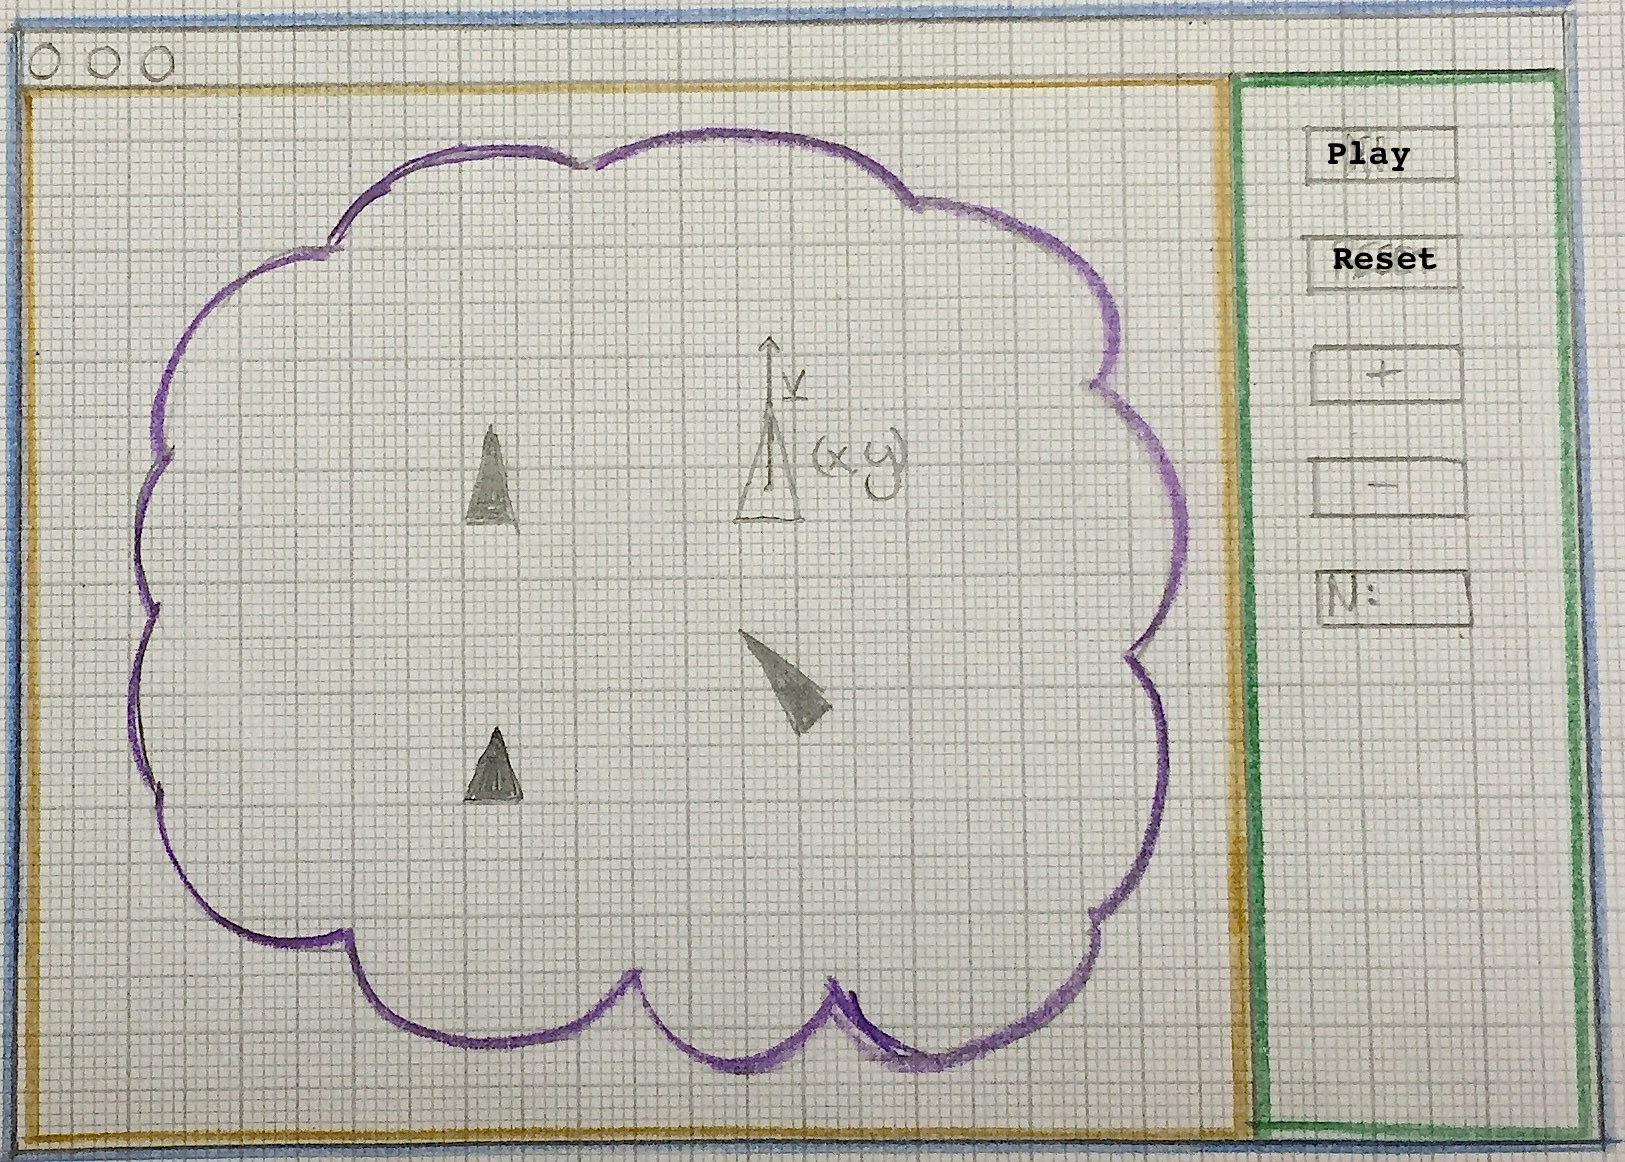
\includegraphics[width = 0.9\textwidth]{images/IdeaSketch.jpg}
  \end{figure}  
  \caption{Initial Sketch of GUI, World, Boids and ``Tools''}
  \label{fig:idea}
  \abovecaptionskip
  \belowcaptionskip
\end{minipage}

\subsubsection{The \code{MainFrame - implements Runnable}}
\label{subsubsec:MainFrame}
This class will contain the applications \code{main}, and will have to set up the different parts of the application, especially regarding the JFrame where everything visible is going to be put. It is going to implement \code{Runnable}, which means the static context can execute in \textit{exactly} two lines of code, leaving the applications objects to interact on their own when it finishes. The last thing this class does in its process to set up the application is to set the JFrame visible, but included in the setup are instantiations of \code{BoidPanel, MenuPanel \& WorldSimulation} as well as making sure necessary communication between them is in place. 

\subsubsection{The \code{BoidPanel - extends JPanel}}
\label{subsubsec:BoidPanel}
This class will be placed onto the JFrame in \code{MainFrame} and will have nothing to do but painting the boids -- acting like a graphical representation of the simulation. It does not need to know about anything but itself and an array list of boids (\textit{and} possibly other objects) to draw.

\subsubsection{The \code{MenuPanel - extends JPanel}}
\label{subsubsec:MenuPanel}
This class will be placed onto the JFrame in \code{MainFrame} together with \code{BoidPanel} and will act like a menu for interaction with the simulation. It will need to have references to both the \code{BoidPanel} as well as the \code{WorldSimulation}, and will have several buttons/sliders/other that makes interaction with the simulation possible( see previous table~\ref{tab:features}).

\subsection{The \code{WorldSimulation}}
\label{subsec:WorldSimulation}
This class will run in the background at all times, and will represent the simulation of the boids. It will need references to both the \code{BoidPanel} and the \code{MenuPanel}, as well as containing an array list of boids and other possible beings. It will monitor the \code{BoidPanel}'s size in such a way that it can mimic the changes done by the panels size change in the simulation. The boids will then be able to have implemented either a ``infinite sandbox mode'' where boids go from one side of the window to the other, or a ``enclosed sandbox mode'' where the boids will repel the walls and stay inside. In the end I decided for an infinite sandbox approach.

\begin{minipage}[T]{0.35\textwidth}
\subsubsection{The \code{Boid}}
\label{subsubsec:Boid}
This class will represent the bird-like object that is going to interact and flock with each other. A boid can be seen as an animal with no knowledge of the world it is in, only its direct environment. It will contain its own position and velocity as well as an array list, containing boids within the neighbourhood, to simulate knowledge of its surroundings. It will for each step of the simulation need to calculate its neighbours, and from that work out separation, alignment and cohesion. The boid will also need to know how to draw itself, but does not need to know in what environment it is drawn in. A graphical representation of a boid is shown in figure~\ref{fig:boid}.
\hfill
\end{minipage}
%
\begin{minipage}[T]{0.65\textwidth}
  \begin{figure}[H]
    \hfill
    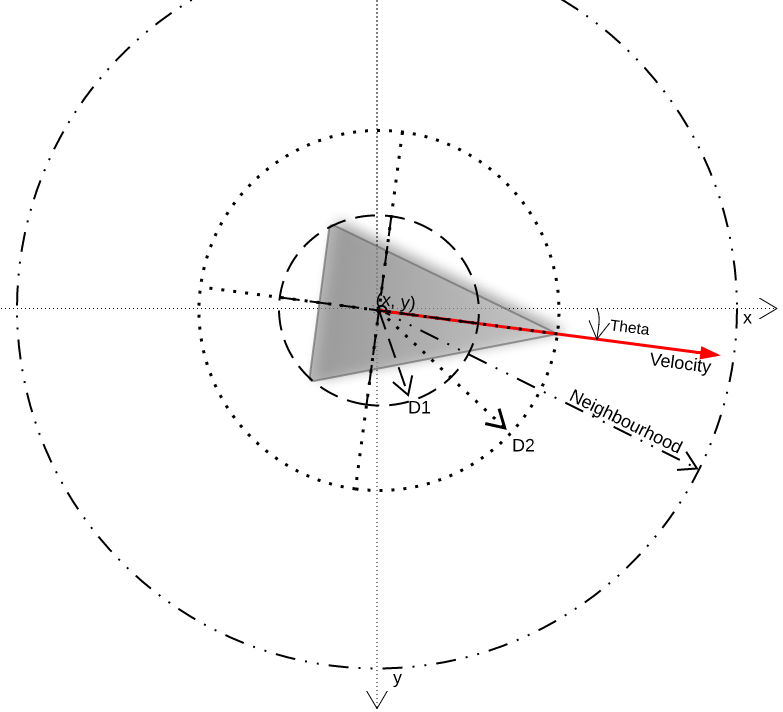
\includegraphics[width = 0.95\textwidth]{images/BoidBuild.png}
    \captionof{figure}{A Boid}
    \label{fig:boid}
    \abovecaptionskip
    \belowcaptionskip
  \end{figure}
\end{minipage}

\subsubsection{\code{Vectors2D} and \code{Coordinates}}

These classes are the lowest levels of abstraction, and both classes are just simple implementation of the Cartesian coordinate $(x,y)$ and a Cartesian vector $\vec{V}^{\,~}$. The vector implementation will simplify the process of dealing with  physical forces, and will have the same compatibility as vectors dealt with in maths/physics: adding, subtracting, scaling and inverting, etc. 

\begin{table}[H]
	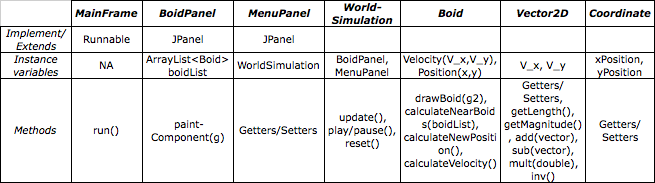
\includegraphics[width=\textwidth]{images/classOverView.png}
    \caption{Classes and Most Important Features}
    \label{tab:classTable}
\end{table}





%----------------------
\section{Implementation}
\label{sec:implementation}
\begin{description}
	\item \textit{To \textbf{``set up''} will in this report be treated as both to instantiate an object in addition to set options, etc.} 
\end{description}

The design process started by putting down every thought on paper, and from there slowly form a plan as to how to write and implement it in code. First thing that was coded was the visible parts -- the GUI. After making a test case and checking that it worked, I then started making my project. Then came the vectors and the coordinates, as these were easily implementable and relatively small. Soon after came the boid class, and as a first I made them draw. After being able to draw them properly, the actual implementation of flocking started. Throughout the writing of the application, several choices regarding placement of code were made. choices were made based on what was cleanest code-wise; for example, it would make sense that the boid itself can calculate where to go next and thus contain the rule-calculations, rather than something else doing this. After implementing the rules and actually seeing boids flock, extra features took place, in addition to simplifying and/or improve already written code. For an overview of each class, see table~\ref{tab:classTable}.

\begin{figure}[H]
  \centering{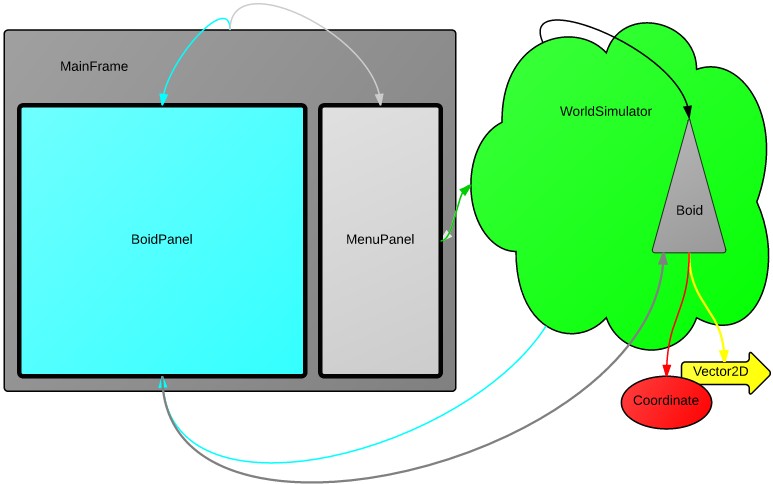
\includegraphics[width = \textwidth]{images/ApplicationStructure.png}}
  \caption{Application Structure}
  \label{fig:applicationStructure}
  \abovecaptionskip
  \belowcaptionskip
\end{figure}

\subsection{A note on doubles}
\label{subsec:doubles}
This is a note on the amazing phenomena in code called \textit{\code{double}}. Since the application is dealing with very specific values at times, especially when calculating values based on $\theta$~(\textit{radians}), and to get rid of any quantisation errors, doubles are used in almost every case. The cases where \code{int}s are used is when there is \textit{no chance} the value can be anything but an integer.

\subsection{\code{WorldSimulation.update()}}
\label{subsec:update}
The world will when instantiated set up references and component listeners, instantiate a array list of boids which it passes to \code{BoidPanel}, and finally it will set up the timer. I had the choice of using \code{Thread.sleep}, or the timer is from the swing-library~($\neq$ utils.Timer). The sleep command will just sleep the current thread, whereas the timer will initially start a separate thread and fire events at a set time interval. For some of the testing, the sleep-method was used, but the timer was implemented for additional features like start, stop and modification of interval. Each timer event will fire a certain set of commands in an anonymous/inner action listener, and will update each boids position, neighbours, velocities, and finally repainting the JPanel. 

\subsection{\code{Boid.calculateVelocity()}}
\label{subsec:flockingImplement}
The boid class is where all the interesting bits are happening! In this class the rules are calculated, the actual boid is moved from one position to another based on its velocity and surroundings, and more. For the boid to be functioning it will need to know which boids in the world are near it, and from that calculate the each rule. For flocking to happen, the rules need to be balanced carefully, and any rule influencing too much/too little will result in the flocking not happening as expected. All rules also has to take special care when there are no boids near, as that sets up for a possible division by 0 in each of the three rules.

\subsubsection{\code{Separation}}
\label{subsubsec:separationImplement}
The separation is a short range force which repels to boids from each other at small distances. The program needed to simulate repulsion, and this is how this repulsion factor got implemented: if any boids are closer than \code{CLOSE{\_}RANGE}, calculate the common position for them all, make a vector in the opposite direction of this point and scale it exponentially to the distance between the boid and the common separation point. This means that if two boids get \textit{very} close together, they will repel each other with near-to-\textit{infinite} force.

\begin{minted}[frame=single, linenos=true]{java}
private void calculateSeparation()
   if(!any_near_boids)
     set separation to 0
   else
     for each boid in nearBoid list
       if(distance between boids are less than "short range")
       add vector from this boid to near boid to totalSeparation
     if(length of totalSeparation is not 0)
       invert and multiply totalSeparation with some exponential factor
\end{minted}

\subsubsection{\code{Alignment}}
\label{subsubsec:alignmentImplement}
The alignment is calculated by taking the the velocity of the surrounding boids added together and divide by the number of boids near.
\begin{minted}[frame=single, linenos=true]{java}
private void calculateAlighment()
   if(!any_near_boids)
     set separation to 0
   else
     for each boid in nearBoids
       add velocities together
     divide total with size of nearBoids, 
     multiply with some factor
\end{minted}

\newpage
\subsubsection{\code{Cohesion}}
\label{subsubsec:cohesionImplement}
The cohesion is calculated by taking an average position of each near boid, and then setting the cohesion to a vector from the boid to that point scaled by some factor.

\begin{minted}[frame=single, linenos=true]{java}
private void calculateCohesion()
   double averageX, averageY;
   if(!any_near_boids)
     set average x/y to the boids position
   else
     for each boid in nearBoids
       add x and y to average x/y
     devide average x/y by the size of nearBoids
   make vector temporaryCohesion from this boid to the average coordinate
   multiply with some factor
\end{minted}

Other dilemmas when it came to implementing the application was simple actions like deciding whether vector handling should be able to coalesce or not -- coalescing would mean being able to do \newline~$\vec{Velocity}^{\,~}$.add(~$\vec{Separation}^{\,~}$.add(~$\vec{Alignment}^{\,~}$.add(~$\vec{Cohesion}^{\,~}$))). Since the application would be dealing with hundreds of vectors each iteration and possibly tens of thousands each second, this would pile up into a \textit{huge} pile of trash~(figuratively speaking) which the \textsc{Java} garbage collector might or might not catch and dispose of, making a lot of valuable memory taken by unused resources. I went for a slightly less modular approach, where instead of making a new vector I would alter the vector instead.

\subsection{File Handling}
\label{subsec:fileHandling}
As time is crucial and this projects due-date got closer, I decided against implementing file handling. The specifications~(Section~\ref{sec:specification}) clearly states that the user should be able to set the number of boids and their starting positions in \textit{some way}. As I have implemented adding boids by mouse click, the user will have an easier time starting the program than any other way. In addition, the add-with-mouse-click in parallel with the sliders for each of the three rules make it possible to recreate a scenario fairly easily and effortlessly again and again, and there is thus no need for file handling. The implementation of it could though be done solely by for each boid storing the position and its velocity, and later feeding that into the application at a later time. The boids would then need a new constructor taking position and velocity as argument.





%----------------------
\section{Testing}
\label{sec:testing}

\begin{minipage}[t]{0.50\textwidth}
The classes mentioned in the design section~(\ref{sec:design}) where tested and implemented step by step, and a process of implementing, testing and perfecting small pieces of code was used for each step, rather than adding overly ambitious amounts of code and then getting lost in hours of error-correction. However, some parts had to be written in parallel with each other or straight into the application, unless a test code the same length of the actual code was used for testing. Testing of directly implemented code was done by adding small amounts of code at a time, debugging the implemented code and checking that it did what it should. Testing was as said done in a variety of ways and especially during the writing of the application, but also near the finish where testing extended to visual pleasantries. The weightings of the different rules are examples of this \textit{visual} testing, and can hardly be done any other way. Figure~\ref{fig:guiANDboidTest} shows how the GUI and the drawing of the boids where checked before starting the rest of the application.
\end{minipage}
%
\begin{minipage}[t]{0.50\textwidth}
    \captionsetup{type=figure}
    \begin{figure}[H]
    	\hfill
      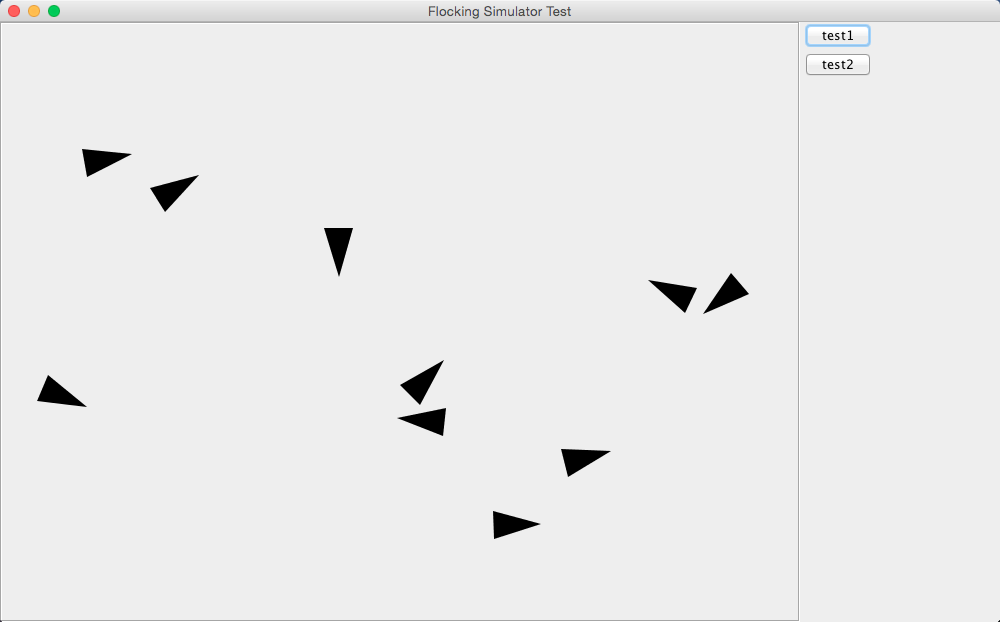
\includegraphics[width=0.9\textwidth]{images/GUITest.png}
    \end{figure}
    \caption{Test of GUI and drawing of boids}
    \label{fig:guiANDboidTest}
    \abovecaptionskip \belowcaptionskip
\end{minipage}

Some examples of different testing can be simple \code{System.out.println("Testing testing")} commands where testing of simple functionality was crucial. The vector class can be an example of this, and was written with a main that tested all the vector calculations(See ``Test'' folder).  After printing results from adding, multiplying, dividing, making, changing and inverting the vectors, it was just a matter of checking the numbers by hand. As long as the numbers matched, testing was considered complete.

In other parts of the application, testing was harder to accomplish by making test code as that would in itself have been complicated. Testing of this was done by debugging parts of the application, exclusively testing only parts of it of the time. Testing of the three rules was done this way. First by writing them, later by running it through a debugger and that checking calculations were sensible, and in the end, the possibly most crucial step of testing the rules; testing it graphically. Actually running it and checking that it looked appealing to the eye was also a crucial step in the process of testing, and several bugs were removed or adjusted. Figure \ref{fig:finalversion} shows a print screen of the finished version, where 100 boids have emergent flocking behaviour.

\textit{Running} the final version, you may notice quite a lot of twitching among the boids instead of smooth transitions and formations. This is due to the fact that the maximum length of the velocity is set rather low, where the rules generate vectors which are much bigger and thus ``takes over''. Reasons for not changing this is because it shows the responsiveness in the boids clearer, and can symbolize the playfulness in \textit{birds} -- which is what we are actually simulating. Changing it would only include making the maximum length of the velocity higher and alter the calculation of the next position in such a way that it went shorter along the velocity vector, and finally adjusting the rules by trial and error until appropriate flocking behaviour emerged again.

\begin{figure}[H]
	\centering
    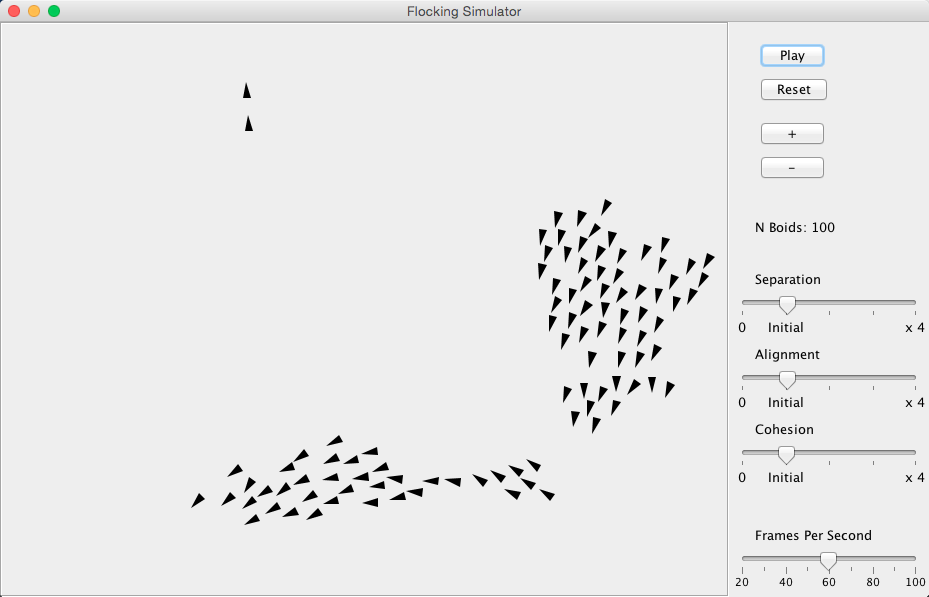
\includegraphics[width=0.9\textwidth]{images/FlockingSimulator.png}
    \caption{Print Screen of the Finished Flocking Simulator}
    \label{fig:finalversion}
\end{figure}




%----------------------
\section{Conclusion}
\label{sec:conclusion}
The application is now finished, although time could have made more of it. Despite everything I am pleased with the result, and have learned a great deal from this project. The product does what it is supposed to do, although there are no such features as predators, obstacles or file handling. When time is available the application will be developed further. As of now, the boids flock with each other due to the rules as they are supposed to, and the application is responsive and easy to use, as well as entertaining. Improvements include predators, obstacles and file handling, as well as the overall resource demand might be possible to decrease. 

%******************************************************************************
%
%		END OF REPORT
%
%******************************************************************************


%%%%%%%%%%%%%%%%%%%%%%%%%%%%%%%%%%%%%%%%%%%%%%%%%%%%%%%%%%%%%%%%%%%%%%%%%%%%%%%
% BIBLIOGRAPHY:
%
% set the style of citations that you want:
\bibliographystyle{plain} % other styles include plain, unsrt, abbrv
%
% generate the bibliography from the .bib file
\bibliography{flockingTex}
%
%%%%%%%%%%%%%%%%%%%%%%%%%%%%%%%%%%%%%%%%%%%%%%%%%%%%%%%%%%%%%%%%%%%%%%%%%%%%%%%


\end{document}